\documentclass[]{../resources/final_report}
\usepackage{graphicx}
\usepackage[hidelinks]{hyperref}
\usepackage{amsmath}
\usepackage[toc,page]{appendix}
\usepackage{wrapfig}
\graphicspath{{../resources/images/}}


%%%%%%%%%%%%%%%%%%%%%%
%%% Input project details
\def\studentname{Roger Milroy}
\def\reportyear{2019}
\def\projecttitle{Autonomous Micro Air Vehicles: Enhanced Navigation in GPS denied environments.}
\def\supervisorname{Professor Sara Bernadini}
\def\degree{BSc (Hons) in Computer Science (Artificial Intelligence)}
\def\fullOrHalfUnit{Full Unit} % indicate if you are doing the project as a Full Unit or Half Unit
\def\finalOrInterim{Interim Report} % indicate if this document is your Final Report or Interim Report

\begin{document}

\maketitle

%%%%%%%%%%%%%%%%%%%%%%
%%% Declaration

\chapter*{Declaration}

This report has been prepared on the basis of my own work. Where other published and unpublished source materials have been used, these have been acknowledged.

\vskip3em

Word Count: 6028

\vskip3em

Student Name: \studentname

\vskip3em

Date of Submission: December 6th 2019

\vskip3em

Signature: Roger Milroy

\newpage

%%%%%%%%%%%%%%%%%%%%%%
%%% Table of Contents
\tableofcontents\pdfbookmark[0]{Table of Contents}{toc}\newpage

%%%%%%%%%%%%%%%%%%%%%%
%%% Your Abstract here

\begin{abstract}

All robotic systems that are mobile require an understanding of their position in order to 
maneuver effectively, avoid obstacles and carry out useful tasks.
In the context of Micro Air Vehicles (MAVs) the situation is more challenging due to the 
twin problems of noisy sensors and limited computation. There are many different approches to 
solving this problem and most if not all of them use the Kalman Filter in order to fuse sensor 
data and provide optimal estimates of state.

%% Objectives
The main objective of this project is to implement the newly proposed technique of 
Hybrid Inference (HI) as an improvement on the Kalman Filter in the context of position 
estimation in MAVs in a simulated environment. The secondary aim is to demonstrate it on the 
DJI Matrice 100 with the Jetson Nano as the onboard computation platform.

The project is based upon a technique of Monocular Simultaneous Localization and Mapping (SLAM) 
which also recovers absolute scale. This integrates visual data and absolute measurments, such 
as Inertial Measurment Unit (IMU) data. It uses an Extended Kalman Filter to integrate the sensor 
data which is what this project will be replacing and evaluating the impact. My initial assessment 
of the Monocular SLAM technique was that the technique was useful but implemented on a specific 
platform, the Parrot AR drone. Upon further investigation I discovered that the implementation
was mostly platform agnostic. This led me to prioritise HI over reimplementing the Monocular SLAM 
technique.

%% Software Engineering approach
The first terms work has not provided much opportunity for applying Software Engineering principles
due to the bulk of the work being that of mastering new theory, learning new technologies and 
assembling existing projects. I was however able to apply them to the design of the architecture of the system as a whole and 
in the HI demonstrator.

%% Background Theory
Monocular SLAM with scale recovery is the technique upon which hybrid inference will be demonstrated. 
Kalman filters are the existing solution and also form the basis of the hybrid inference solution,
as it uses the same problem formulation. HI is the general technique that fuses existing 
mathematical techniques with neural networks. The report explores both theoretical and technical 
aspects of all these techniques.

%% Work Completed
The report details a summary of the work that has been completed this term. Learning how to
use ROS and Gazebo, setting up the TUM ardrone and hector packages that I am building upon. 
And finally, implementing a demonstrator of the HI technique on a synthetic dataset. 

%% Second term work.
Some additional challenges have been identified during the course of this work. First is that HI as described 
in the paper, deals with a simplified linear dynamic model that does not have inputs to the system.
The dynamic model that describes MAVs must include external inputs for control. Reformulating the 
graphical model to account for this is the first new challenge that I had not identifiend in the 
initial project plan. The second challenge is temporal. With a Kalman Filter, it is possible to 
estimate future states and the uncertainty of those postulated states. This is critical for dealing 
with latency issues in the real time control environment that MAVs present. The current formulation 
of the underlying graphical model does not allow for future reasoning, solving this is necessary to
enable HI to be used this domain.

Finally I describe the work to be completed in the second term. The provided Gantt chart shows the
projected timeline.

\end{abstract}
\newpage

%%%%%%%%%%%%%%%%%%%%%%
%%% Introduction
\chapter{Introduction}


%%%%%%%%%%%%%%%%%%%%%%
%%% 
\section{Motivation}

Micro Air Vehicles (MAVs) popularly known as quadcopters, have become ubiquitous in recent years 
with prices dropping across a range of sizes of drones. This has lead to their deployment across 
a number of sectors and applications. These include videography, where most of us will have seen 
their output, all the way to assessing and counting endangered species with numerous other 
applications in between.

One major challenge is that of fixing position accurately. Most solutions use some kind of 
satellite navigation solution to fix absolute position. This is effective in outdoor environments
but ineffective in a number of environments, such as anywhere indoors, in forests or underwater.
In these environments it is necessary to rely on inertial sensors as well as image or other data. 
These are fused in an Extended Kalman Filter to produce a single estimate of position.
The main issue with these techniques is that absent regular fixes of known positions, estimates of
position accumulate error.

If we can reduce the rate that this error accumulates, this opens up the space of viable environments
that automated systems can operate in and increases their usefulness.


%%%%%%%%%%%%%%%%%%%
%%% Objectives
\section{Objectives and Contributions}

\subsection{Objectives}
The main objective is to apply the newly proposed technique of Hybrid Inference (HI)
\cite{HybridInference} to the problem of position estimation in MAVs. HI integrates 
existing mathematical models with Neural Networks in order to improve inference performance in 
both low and high data regimes.

In addition I aim to demonstrate HI using onboard computation, taking position estimates that 
come from inertial sensors and visual SLAM systems. I will use a Jetson Nano for computation, 
mounted to a DJI Matrice 100 quadcopter.

For the first term, the key objectives were to validate the technique by implementing it on a 
small synthetic dataset, to demonstrate in Gazebo the Monocular SLAM with scale recovery technique 
\cite{Engel:Camera-basedNav} upon which the Hybrid Inference will be implemented and finally to 
validate the Jetson Nano platform for computation. All these objectives were successfully achieved.

The objectives for the second term are to implement Hybrid Inference for state estimation completely 
and demonstrate it on a simulated quadcopter in Gazebo. Secondary goals are to integrate the 
Jetson Nano onto the Matrice 100 and adapt the code to work with the DJI OSDK. Finally to demostrate 
the fully realised project in precision figure flying in order to compare with the results of 
Engel et al. \cite{Engel:FigureFlying}.

% \subsection{Contributions}
% To apply this technique to a new problem instance and to evaluate whether it improves on current 
% state estimation techniques. To suggest its viability for onboard deployment on resource constrained
% platforms.

%%%%%%%%%%%%%%%%%%%%%%
%%% Planning and Timescale
\chapter{First Term Planning}

\section{Original Plan}

The original plan delayed the bulk of the implementation until the second term. While this was 
not unreasonable given the learning curve for each of the technologies involved, if I stuck to 
the original plan I would have been faced with a huge amount of work with little to base it on.
There was also quite a lot of uncertainty about the state of the TUM codebase. The original 
assumption was that the code had been written specifically to work with the Parrot AR drone as 
it was the platform on which they demonstrated \cite{Engel:Camera-basedNav}.
This would have meant rewriting the code to work in ROS and be platform independent. When I found 
that was not the case it changed the dynamics of the project quite significantly and led to the 
new plan.

I have included below the original plan Gantt Charts that detail milestones and timescales.
\\
% Gantt chart?
\begin{figure}[h]
  \centering
  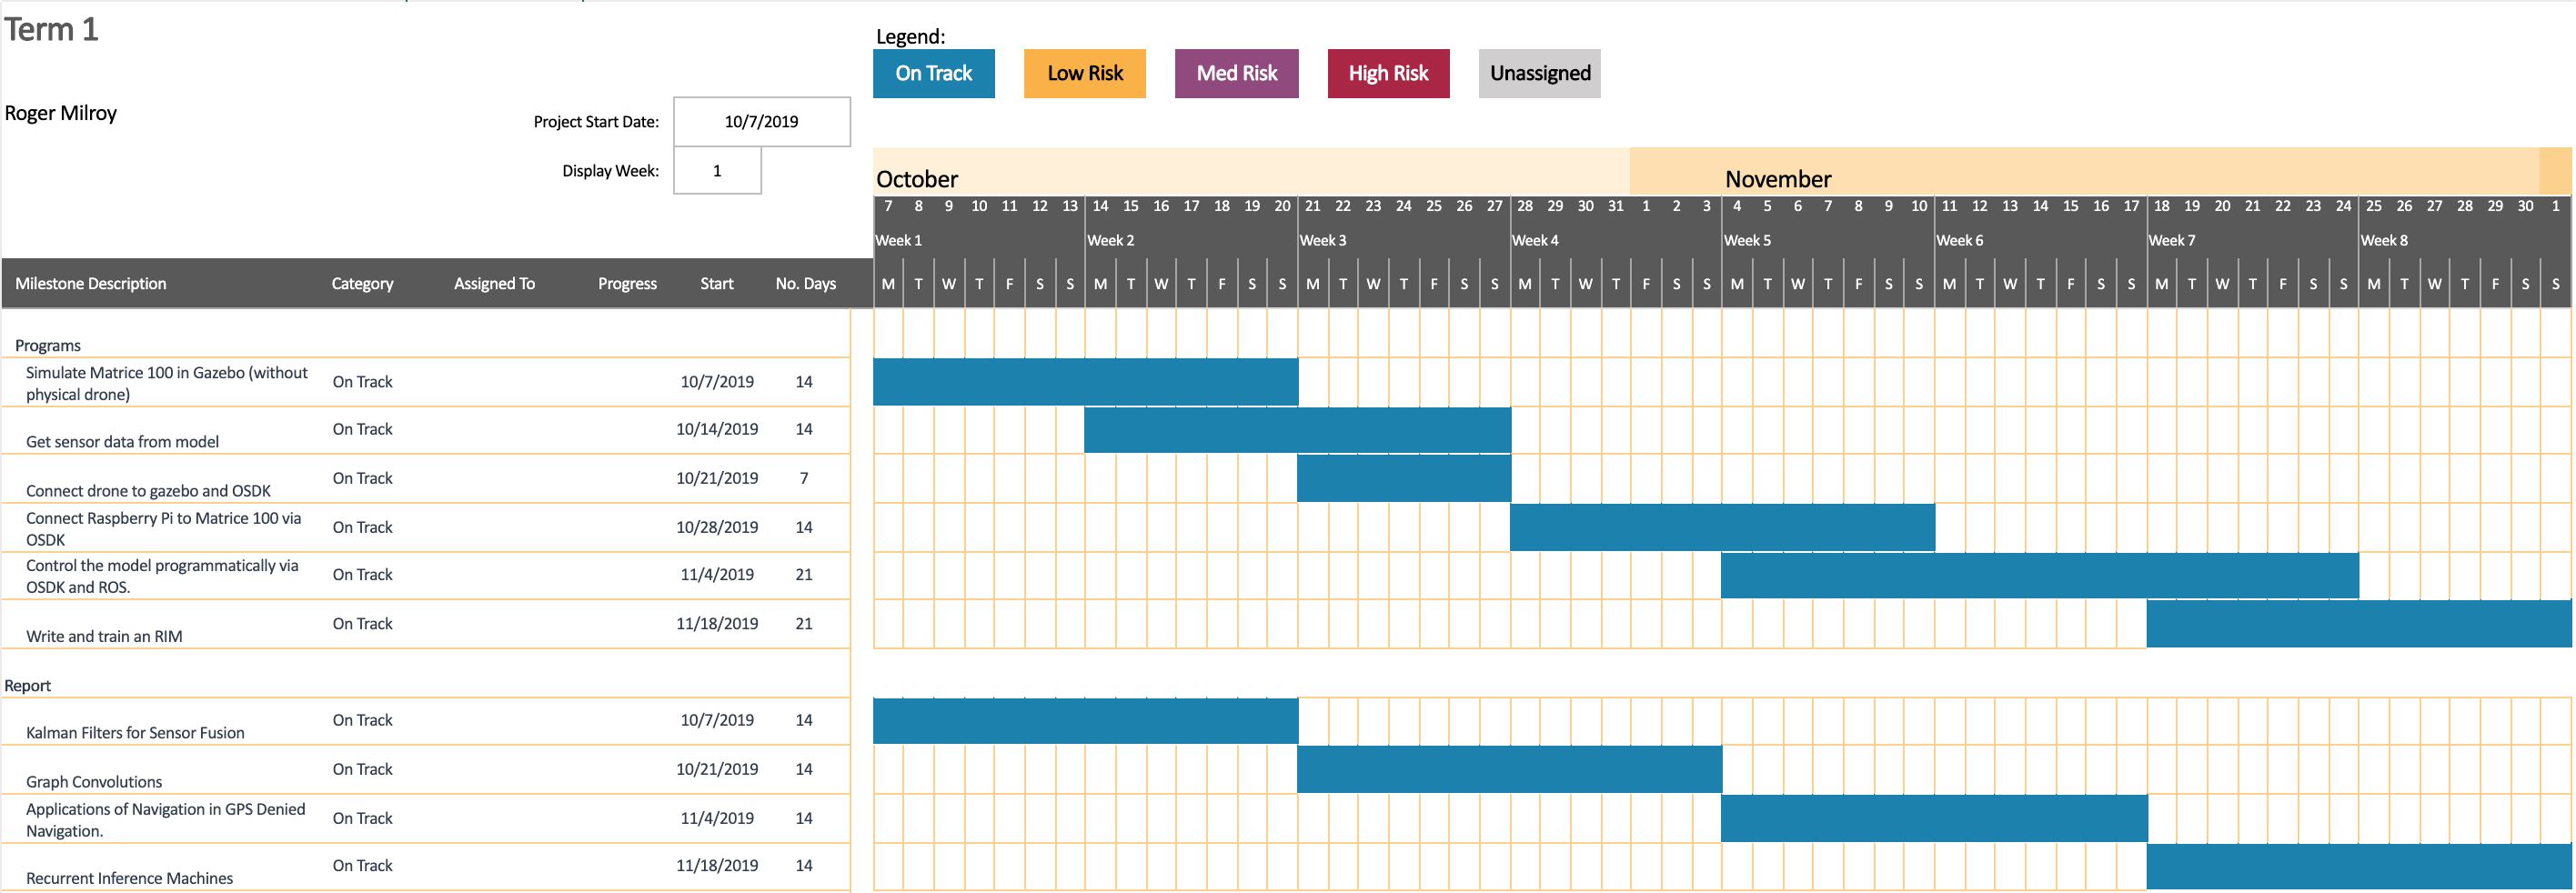
\includegraphics[width=\textwidth]{Term1Ganttv1.png}
  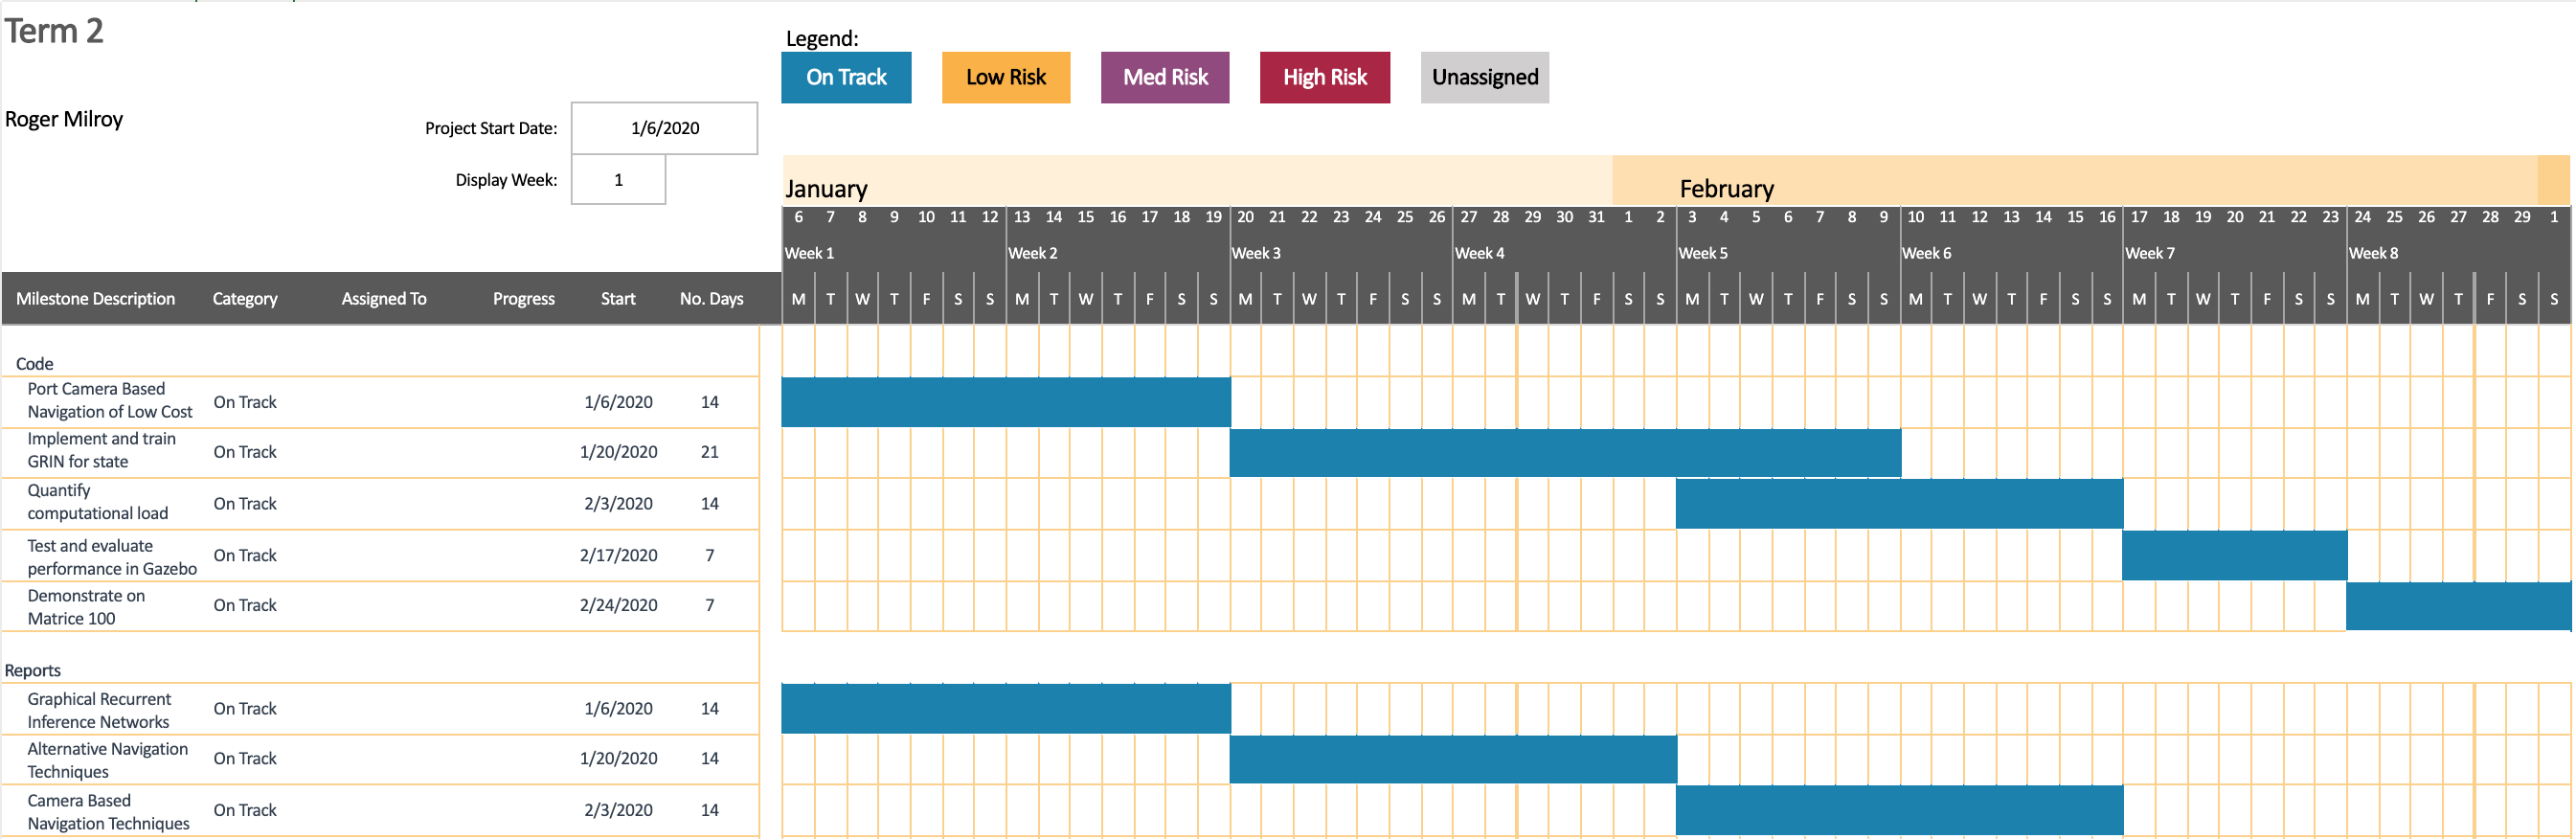
\includegraphics[width=\textwidth]{Term2Ganttv1.png}
  \caption{Original Plan Gantt Charts}
  \label{}
\end{figure}


\pagebreak
\section{Revised Plan}

While working on the project the outlook changed quite significantly when I found the code for 
the Monocular SLAM with scale recovery was open source. This meant that I could directly build 
upon their work and extend it instead of spending the bulk of the project reimplementing their 
technique. This enabled me to pivot to focusing more on the implementation of HI. 
Under the new plan most of the first term is spent getting simulation working with the existing 
code base. I also implement a simple version of the HI technique on synthetic 
position data.

I replanned and the following are the updated milestones and associated dates. I will elaborate 
on the work to be done in the second term at the end of the report.
\\
\begin{figure}[h]
  \centering
  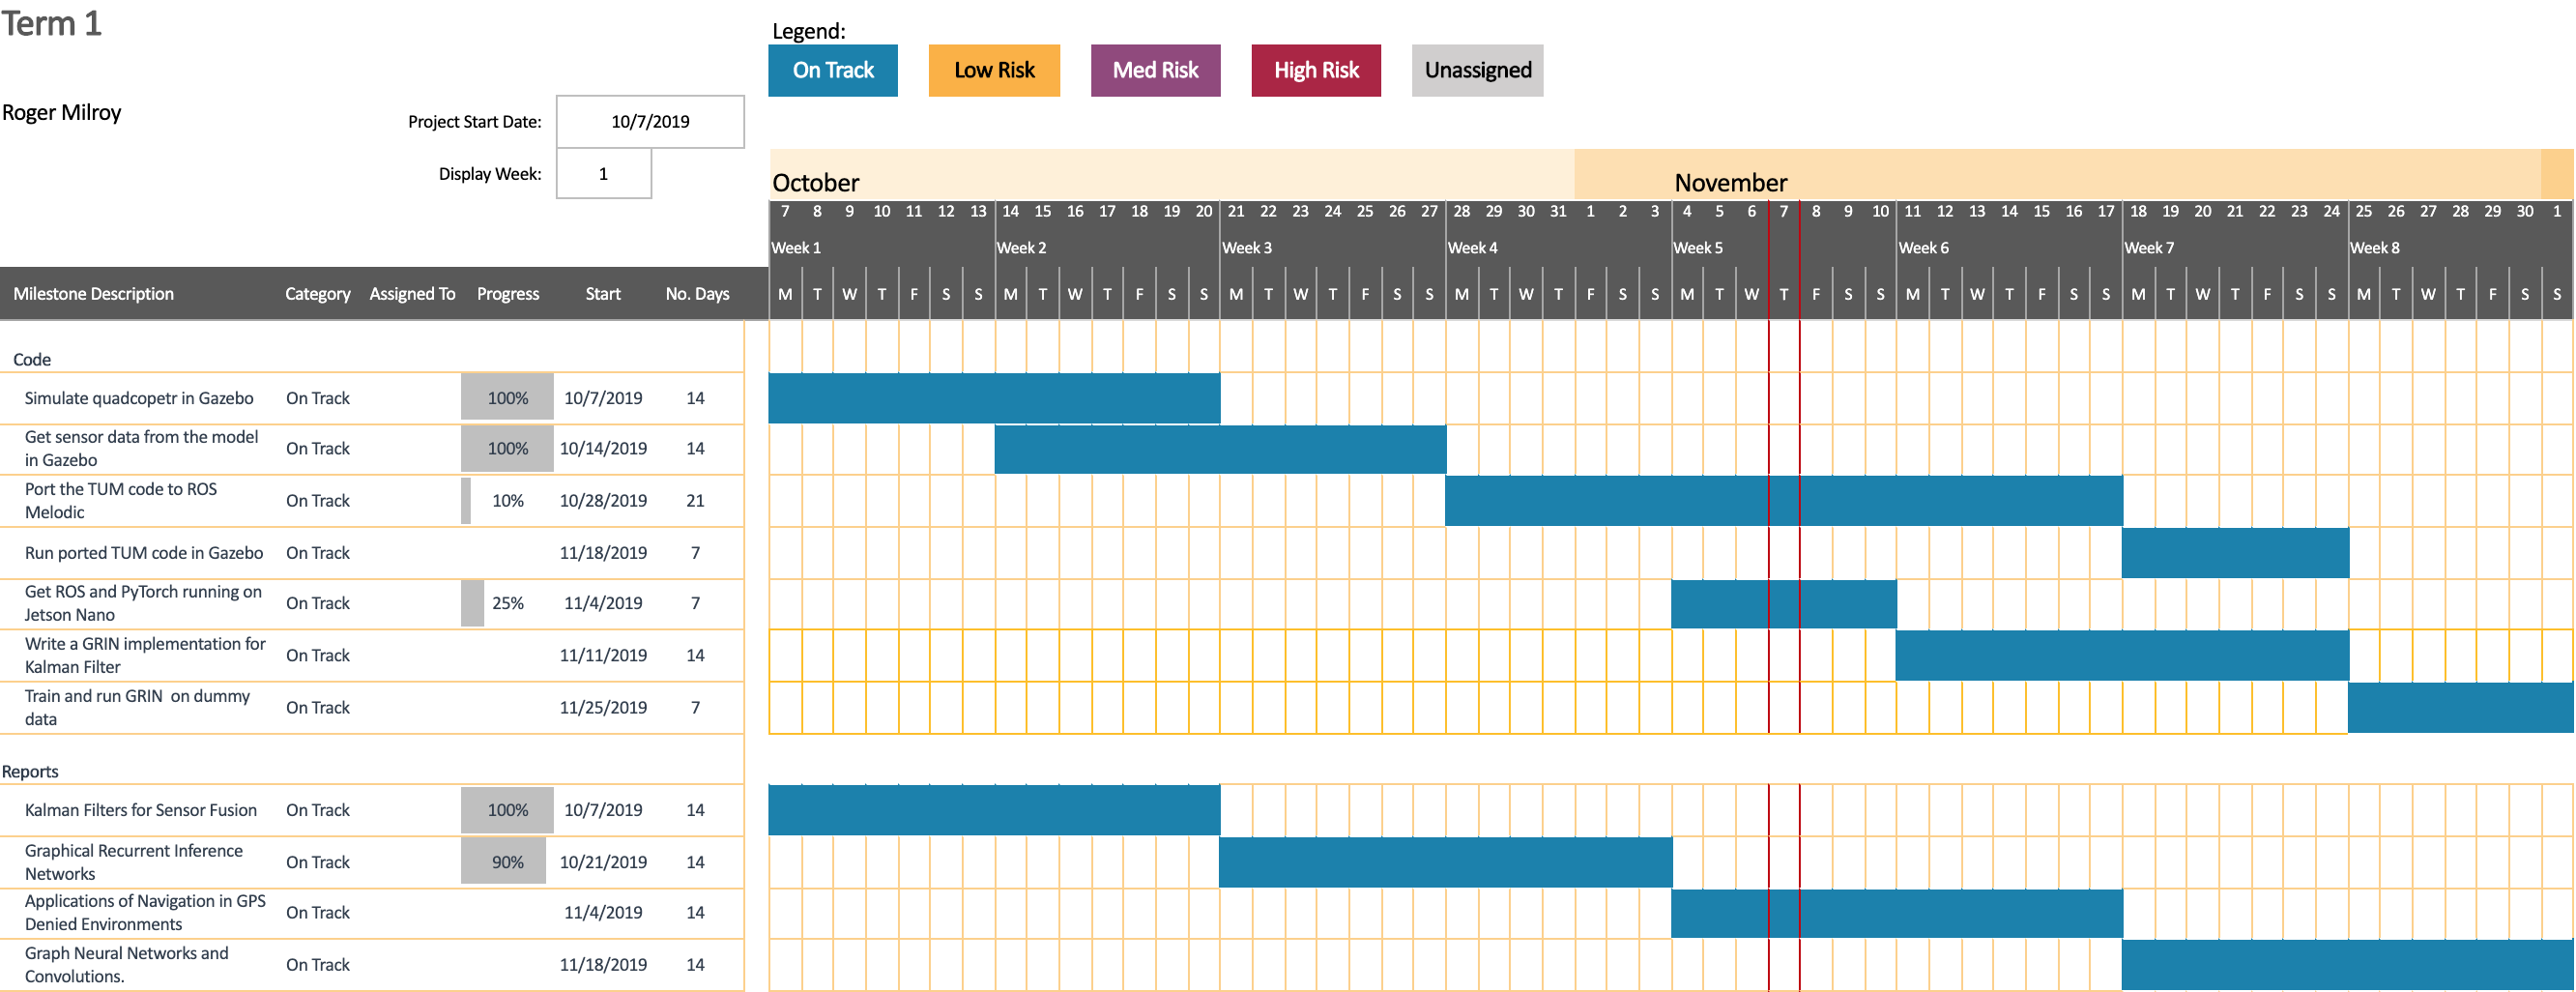
\includegraphics[width=\textwidth]{Term1GanttChart.png}
  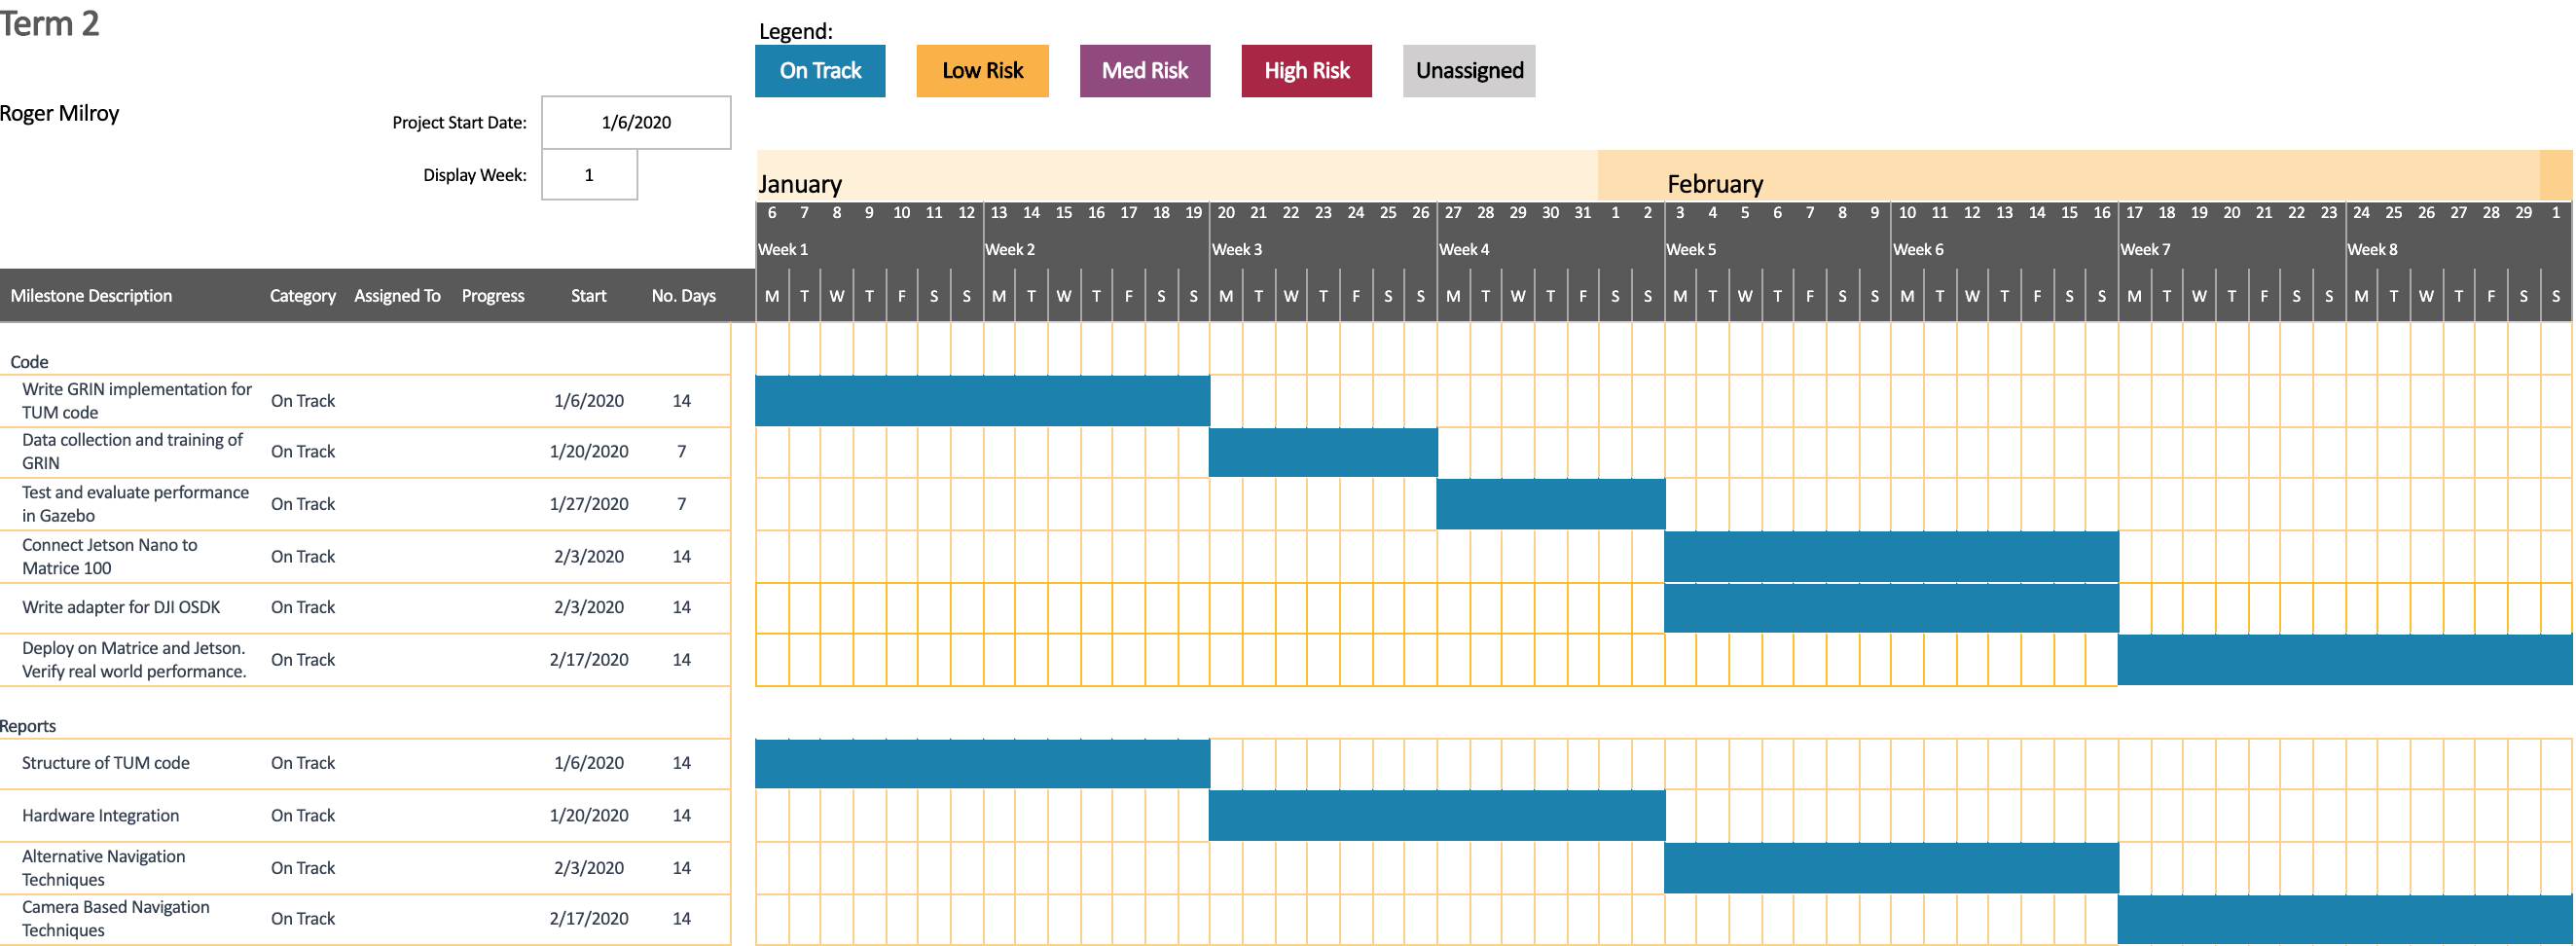
\includegraphics[width=\textwidth]{Term2GanttChart.png}
  \caption{Revised Plan Gantt Chart}
  \label{}
\end{figure}


%%% Software Engineering
\chapter{Software Engineering}

\section{Tools}

\subsection{Version Control System}
I used git as my version control system, and GitHub as my remote. I actually have a number of 
repositories because for the ROS section of the project it was necessary to modify existing 
projects code. I created a private fork of the relevant projects and then modified them as necessary.

I have separate branches for development, reports and for each feature that I am working on. 
These last ones are only temporary and are closed as soon as the feature is tested and integrated 
back into development. The workflow that I have decided upon is to use development for completed 
features once they have been tested. This does not imply that development is stable however so I 
only release code considered stable to master. The idea is that master should only contain stable 
code and be safe to use at any point.

\subsection{Project Task Tracking}
I used Trello in order to organise and keep track of tasks while completing them. I use a single 
board with To Do, Doing and Done lists. Each task is a card and has an associated due date.
This is really useful to stay on track and quickly assess the state of the project at a glance. 
I also used this while replanning as I could evaluate each task and see whether it was still 
relevant in the new context. One additional advantage of using Trello is that it keeps track of 
history and has space for lists within tasks allowing them to be broken up into sub tasks.


\subsection{Development Tools}

I used both VSCode and PyCharm as Development Environments. They both have different advantages 
and disadvantages and I used VSCode for the C++ work and PyCharm for the Python work.
For ROS development I have an Ubuntu VM with the relevant dependencies installed as well as the 
two IDEs I just mentioned.

I used the built in testing framework for Python, 'unittest' for testing. This provides a very 
similar framework to JUnit and allows for clear easy test setup and management.

\pagebreak
\section{Development}

\subsection{Design}
% ROS
ROS lends itself to modular code however the packages that I am working with and building on have 
very mixed engineering approaches. To date my work has been composing the projects and getting them 
to run so Software Engineering practices have been limited to thinking about the design of the full 
implementation.

Unfortunately ROS is not particularly conducive to Test Driven Development (TDD) as there is no 
framework that enables testing outside of nodes. I can test the components of each node in the 
standard fashion, which I plan to do though this will apply more next term.

All of the design decisions that I have taken, both for implementations this term and the plans 
for future work, have been in the pursuit of modularity.

It is widely accepted that good code should be modular and reusable where possible. There are 
aspects where this is obviously not possible, such as configurations and any implementation 
specific work, but this should where possible be isolated and offer abstract interfaces.

With respect to the packages I have chosen, the hector stack and the TUM work, they have to some 
extent taken this approach but only really within the project. 
This complicates my work somewhat but at the same time using these as the base allows me to explore
 more advanced concepts over reimplementing the functionality of these modules.
I will be writing adapters to enable the existing codebase to interact.

For the proof of concept of Hybrid Inference, the Dataset and the Linear Motion Model that creates 
synthetic data I implemented them as separate classes. A standard Object Oriented approach and used
composition where necessary.


\subsection{Testing Strategy}

Due to the limitations that I have regarding support for testing frameworks, particularly in ROS, 
I have relied a lot on sanity checking at each stage while testing formally as many sections as 
possible. Integration tests are particularly important for my project as I have a variety of 
different technologies that need to work together across a number of interfaces.
This will become important in the next stage of the project as that is when the different components 
start to interact and when I will be looking to start deploying code onto the hardware.

To this point I have thoroughly Unit Tested the proof of concept of HI, the 
Dataset and Linear Motion model.

\pagebreak
\subsection{UML}
%% UML
I have included the package diagram that describes the high level design 
of the project as well as the class diagram of the HI demonstrator.

\begin{figure}[h]
  \centering
  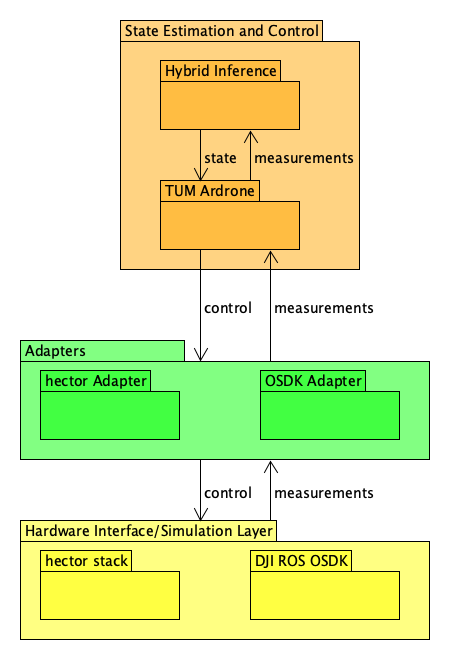
\includegraphics[height=0.30\textheight]{hybrid-inference-package-uml.png}  
  \caption{Package diagram of the project.}
  \label{}
\end{figure}


\begin{figure}[h]
  \centering
  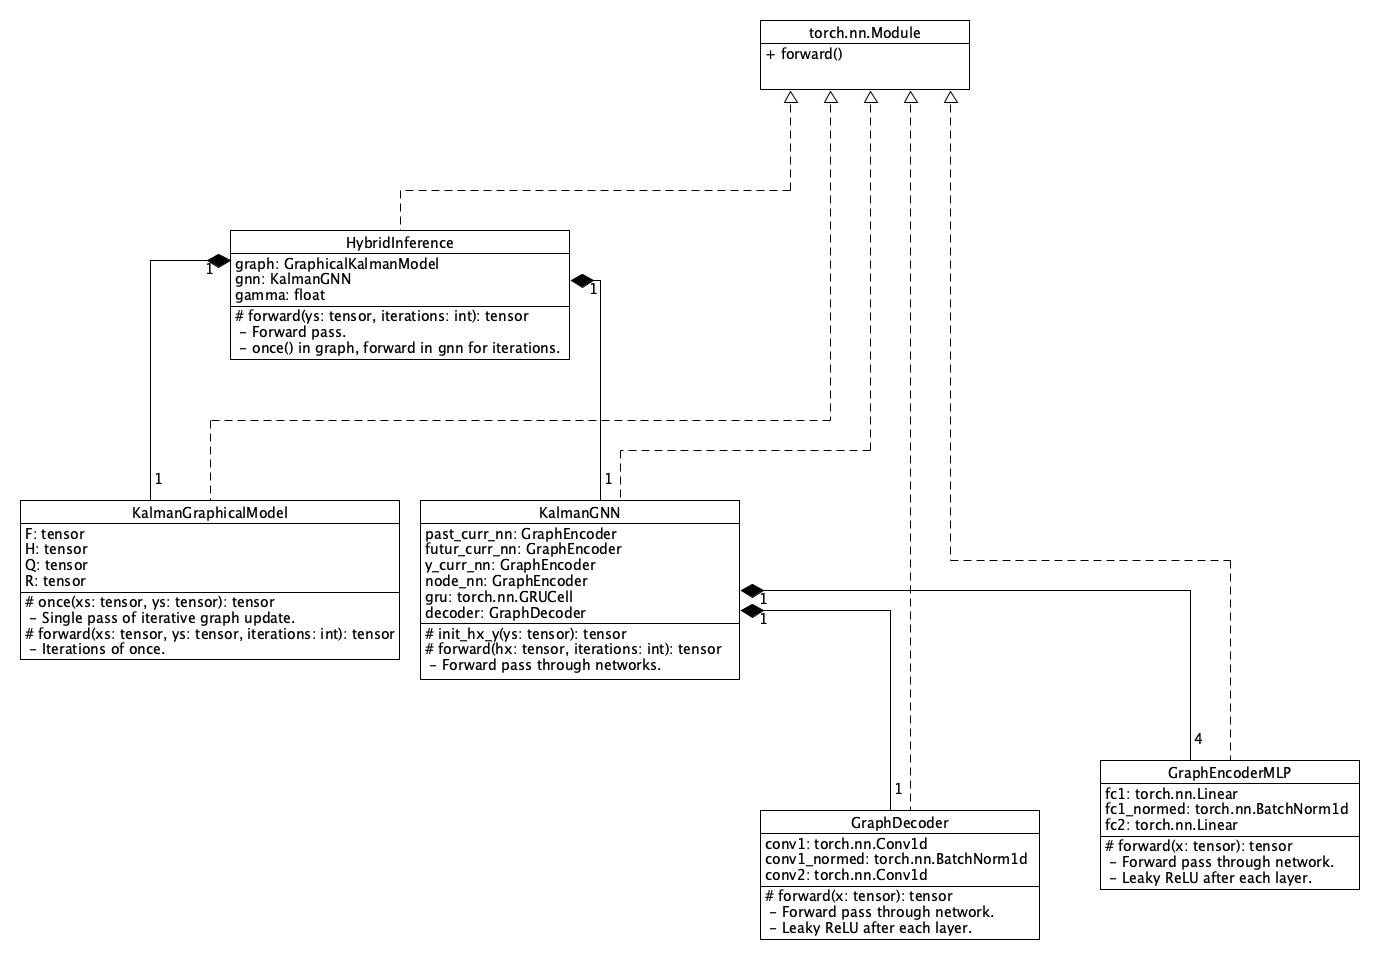
\includegraphics[height=0.36\textheight]{hybrid-inference-uml.png}
  \caption{Class diagram for Hybrid Inference}
  \label{}
\end{figure}


%%%%%%%%%%%%%%%%%%%%%%
%%% Literature Review
\chapter{Background Theory}
% This is where the background theory will go too.

\section{Gazebo and ROS}

%% Explainer on Gazebo and ROS and see if there are references for them.
In order to demostrate the effectiveness of the code that I have written it is essential that it is 
demonstrated first in a simulated environment. This neccesitates using Gazebo as it is the industry 
standard robot simulation software. In a similar token the industry standard robot development 
framework is ROS, which works with Gazebo and so this is the primary technology stack that I am 
using.

Both ROS and Gazebo are very powerful but they don't have a particularly easy onboarding process. 
For learning basic ROS concepts I used a service called Robot Ignite Academy that has some simple 
tutorials to make the process of learning the ROS way of doing things a bit quicker. One challenge I 
had at the very early stage was understanding what ROS actually was. There are very few high level 
descriptions of it, and they are certainly not the first topic on the ROS tutorials pages.

What I learned was that ROS is a paradigm of programming robots as well as an 
implementation of that paradigm. The paradigm is that each peice of code on the robot is a Node 
that takes data from a Topic, processes it and outputs data for other Nodes to use on a Topic. 
Some Nodes don't do both of these and some also directly effect change in the robot, think of a 
Node that controls a motor, it would read and change the voltage to the motor.

The other concepts that make up ROS are that of Services which are synchronous and Activities that 
are asynchronous, both operate on the Client - Server pattern. Topics as I mentioned are 
communication channels that operate on the Publisher-Subscriber pattern. And Messages which actually 
have quite a bit of intricacy and can be quite confusing. There are 3 types of Message. Regular 
Messages that are published to Topics. Then Actions and Services also define their own formats of 
messages. They will often use standard messages defined for use in Topics but additional message 
formats will be generated for each Action or Service.
%% Need to add references

\section{Monocular SLAM with scale recovery.}

%% put a UML diagram of the library layout/dependancies.
In two related papers \cite{Engel:FigureFlying}\cite{Engel:Camera-basedNav}, Engel et al. present a 
technique of Monocular SLAM that is able to recover absolute scale. In order to understand why 
this is significant and important some background is needed.

The primary problem of visual SLAM techniques is that of creating a high quality depth map of the 
surroundings. This can be accomplished by stereo vision, which is where two cameras are used and the 
distance and rotation between the two of them are known. Ideally the axes are aligned and there is 
no rotation between the cameras though this can vary depending on the specific requirements.
This can be extended to use three or more cameras but in the more general case, known as structure 
from motion, it is possible to use a single camera. In that case we are trying to recover the 
transformation and rotation between frames. This is possible however it is not possible to recover 
absolute scale from this technique as we don't know the absolute distances between frames. In the 
stereo case the information about the position and orientation of the cameras relative to each other
is known a priori and so we can recover absolute scale.

Engel et al. tackle the issue of scale recovery by using data from the IMU which usually consists of 
3 accelerometers and 3 gyroscopes and often a magnetometer or other absolute scale sensors such as 
altimeter or barometer. This is standard equipment on quadcopters as it is needed to maintain stability. 
They use the information provided by this sensor in conjunction with the structure from motion 
equations in order to recover the absolute scale. In order to estimate the scale factor which is 
usually referred to as $\lambda$ they take a maximum likelihood approach, which in simple terms 
means they estimate the $\lambda$ that maximises the likelihood of the $x$ and $y$ positions 
measured by onboard sensors. In order to solve successfully they turn it into the negative log 
likelihood which you then minimize. This is a common trick and in this case it leads to a closed 
form solution for $\lambda$. This is important as it reduces the computational cost and makes it 
more feasible with onboard computation. In the paper they use a Parrot AR drone which has very 
constrained payload and computation capacity so they use offboard computation.

In the second paper \cite{Engel:FigureFlying} they present the full system including the scale 
estimation and demonstrate its effectiveness in position flying and holding.


\section{State Estimation}

%% Kalman Filters
The core method used for state estimation in the face of noisy sensors is the Kalman Filter. It is 
used by Engel et al.\cite{Engel:Camera-basedNav} for state estimation and sensor fusion which are 
its most common uses in this field.

Let us formally define the problem. The system we are measuring is assumed to be characterised by a 
Hidden Markov Model, this is how Kalman characterised the dynamical system we are interested in \cite{Kalman1960ANA}. 
In this formulation there are hidden states $x$ and observations $y$. The system being a Hidden 
Markov Process means that it is characterised by the following equations:

\begin{align}
  x_t &= Ax_{t-1} + Q_t \\
  y_t &= Hx_t + R_t
\end{align}

Where $A$ is the transition matrix from time $t-1$ to $t$, and $\xi_t$ is the noise at time $t$. 
This represents that the model dynamics are stationary so $A$ is fixed but there is noise in 
transitions, that is transitioning between states is non-deterministic. $H$ is the measurement 
matrix and $R_t$ is the noise in the measurements. This models the reality of noisy measurements 
that may not be correct and in fact represents the true problem. We want to recover the true 
measurements despite being given noisy observations.

The Kalman Filter gives an optimum estimate of $x$ which I will call $x^*$ by deriving three matrices 
$\Phi^*$, $P^*$ and $\Delta^*$:

\begin{align}
  \Delta^*(t) &= A_{t+1;t}P^*_tH^T_t[H_tP^*_tH^T_t]^{-1} \\
  \Phi^*_{t+1;t} &= A_{t+1;t} - \Delta^*_{t+1;t}H{t} \\
  P^*_{t+1} &= \Phi^*_{t+1;t}P^*_tA^T_{t+1;t} + Q{t}
\end{align}

\pagebreak
Note that in the Kalman formulation he also considers non stationary dynamic systems. In our 
situation we assume stationarity which allows us to drop the time specification on the transition 
matrices $A$ and $H$.

With these matrices, the optimal estimate of state at time $t+1$, $\hat{x}_{t+1|t}$ is given by 

\begin{align}
  \hat{x}_{t+1|t} &= A^*\hat{x}_{t|t-1} + \Delta^*_ty_t
\end{align}

The estimation error $x'$ and covariance of the error, cov $x'$ are

\begin{align}
  x'_{t+1|t} &= A^*x'_{t|t-1} + Q_t \\
  \text{cov } x' &= P^*_t
\end{align}

From this we can see that the Kalman Filter is an iterative process where each iteration builds upon 
the previous best estimate of state. To recover the estimates of the true measurements we simply 
need to multiply the best estimates of the state by the measurement matris $H$.

Kalman and Bucy extended the Kalman filter that, in the form stated above works for discrete time, to the 
continuous case the year after the original paper \cite{Klmn1961NewRI}.

These equations only apply to linear dynamic models which is something of an issue given that most 
real life applications are of non linear dynamic systems. To solve this we use Taylor expansions to 
linearise our non-linear models around the current state \cite{ExtendedKalmanNasa}. This does 
unfortunately add a large overhead as we need to re linearise at each time step to avoid 
accumulating linearisation errors.

%% Hybrid Inference
\section{Hybrid Inference}

Now I introduce the technique that form the core objective of this project, Hybrid Inference. First 
introduced in \cite{HybridInference} which also gave examples on Lorenz attractors and 
Kalman filters. While Kalman Filters give optimal estimates in the face of noise, it is almost 
impossible for them to be completely precise due to that noise. This we can see by observing the 
error in the estimates at each time step.

Absent an accurate fix of state, ie. a noiseless measurement, the error grows 
continuously to the point where estimates may no longer be meaningful.

At the same time it is now possible to train a neural network to directly estimate position given
noisy inputs \cite{NNStateEstimation}. The concept of Hybrid Inference is to leverage the relative 
strengths of pre-existing knowledge, in this case the Kalman Filter that accurately describes the 
behaviour of linear or linearised dynamic models up to a degree of error, and Deep Learning techniques 
that are able to model highly non linear systems but require large amounts of data to train.
In the Hybrid Inference model, expert knowledge is incorporated by integrating the model of the 
system with a Graphical Neural Network (GNN) modelling the residual error to improve accuracy above what is possible with a 
Kalman filter alone.

\pagebreak
Reexamining the problem solved by the Kalman filter, Satorras, Akata and Welling reformulate the 
problem to be a maximum likelihood problem \cite{HybridInference}.
Where the states are $\mathbf{x} = \{x_0, x_1 ... x_k\}$ and the observations are $\mathbf{y} = \{y_0, y_1 ... y_k\}$
In this context, the task is to predict the optimal estimate of $\mathbf{x}$, $\mathbf{\hat{x}}$ which is defined as

\begin{align}
  \mathbf{\hat{x}} = \underset{x}{\text{argmax}}\ p(\mathbf{x}|\mathbf{y})
\end{align}

Again as we assume a Markov process and that the transition is stationary this can be expressed as 

\begin{align}
  p(\mathbf{x},\mathbf{y}) = p(x_0)\prod_{t=1}^T p(x_t|x_t-1) p(y_t|x_t)
\end{align}

They model this as an iterative optimization process to arrive at $\mathbf{\hat{x}}$
Specifically they define a recursive update operation for the general case and then formulate it 
for the Hidden Markov case

\begin{align}
  x_t^{(i+1)} = x_t^{(i)} + \gamma M_t
\end{align}

Where $M_t$ represents the sum of matrix products, which they call messages, from $x_t-1$ to $x_t$ 
from $x_t+1$ to $x_t$ and from $y_t$ to $x_t$.

In our case these messages turn out to be

\begin{align}
  x_{t-1} \rightarrow x_{t} &= -Q^{-1}(x_t - Fx_{t-1}) \\
  x_{t+1} \rightarrow x_{t} &= F^TQ^{-1}(x_{t+1} - Fx_t) \\
  y_t \rightarrow x_t &= H^TR^{-1}(y_t - Hx_t) 
\end{align}

% \begin{wrapfigure}{r}{0.25\textwidth} %this figure will be at the right
%   \centering
  
% \end{wrapfigure}

The graphical interpretation is of the $x$s and $y$s at each time step forming nodes in a graph. The 
edges are the same as the direction of the messages, that is from $x_{t-1} \rightarrow x_t$, $x_{t+1} \rightarrow x_t$ and $y_t \rightarrow x_t$. 
The messages passed over these edges iteratively update the $x$s and after some iterations they 
converge to a best estimate.

%% Insert a graph here.

\begin{figure}[h]
  \centering
  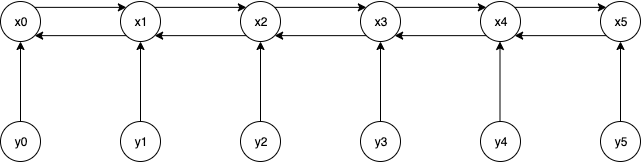
\includegraphics[width=0.8\textwidth]{GraphicalKalmanModel.png}  
  \caption{}
  \label{}
\end{figure}




This graphical interpretation allows us to define an equivalent graph with different dimension nodes 
but the same edges. These are known as $h_x$ and $h_y$ which stands for hidden nodes relating to $x$ 
and $y$ respectively. 

%% Insert another graph here.

The key part of the paper is to define a GNN that operates over this graph with a message passing
routine over the nodes that connect edges and the messages passed in the original 
graph. More specifically for each type of edge, for example $y_t \rightarrow x_t$, we define a 
feedforward neural network that takes the source node, the target node and the message and outputs 
an encoding of the edge, I will refer to these as edge models. These encodings are summed according 
to their source node and then passed through a separate feedforward network which I will call the 
node model. 

The output of this is passed through a Gated Recurrent Unit (GRU) along with the 
previous $h_x$ in order to produce a new estimate of $h_x$. The interpretation of this is that 
edge feedforward networks compute the residual error over the edges, the node model computes the 
residual error left in the $h_x$ and the GRU allows some of the past residual error to propagate 
into the current estimate. The final step passes the new $h_x$ through a decoding step to produce an additional corrective 
factor in addition to $M_t$ called $\epsilon$.

This gives us the final general recursive update rule

\begin{align}
  x_t^{(i+1)} = x_t^{(i)} + \gamma (M_t + \epsilon_t)
\end{align}


%%%%%%%%%%%%%%%%%%%%%%
%%% Work Completed
\chapter{Work Completed}

%%% Written Summary
\section{ROS and Gazebo}

%% install ROS and Gazebo
The first task to carry out was to install ROS and Gazebo. As mentioned earlier ROS is the framework 
into which my code will fit. Gazebo is a simulation tool that I will be using to verify everything 
before deploying anything in reality. Luckily Gazebo is included with ROS (with some exceptions) so 
installing it separately is not necessary. If you need the most recent version of Gazebo this is not 
true, you need to follow some additional steps to install it and link it with ROS so they interact 
correctly.

I did have some confusion about which version of ROS I needed to be compatible with various things 
but I made the decision to stick with the most recent version of ROS and the standard version of 
Gazebo packaged with that. This simplifies the setup for anyone seeking to reproduce my project.

The ROS website\cite{melodic/installation/ubuntu} has an excellent guide on installing ROS for the 
first time on Ubuntu and I highly recommend it.

%% install hector code

%% explain catkin workspace.

After that I installed the hector stack. This was quite a long process of trial and error as there 
does not seem to be a guide for getting started with this set of packages. I first tried to install 
them from apt as they are available there. That did not work and I believe the issue is that they 
were built for an earlier version of ROS but packaged for melodic without any changes. Regardless 
of the reason that did not work. I was trying to install the hector quadrotor and hector gazebo 
packages as those were the only packages that I believed that I needed. I tried to clone them into 
the src folder of my catkin workspace. While trying to build it failed because of dependencies on 
other hector packages, namely hector slam hector models and hector localization. Then it was missing 
the geographic mesages. Then it failed because it was missing qt4. I installed both of those with 
apt. The full process took a while longer than this explanation as you only find out anpther 
dependency is missing after building again. A final issue was that the memory usage at certain 
points spikes. It turned out that this was causing the VM to run out of memory and stop compliation. 
This caused very confusing error messages as they didnt seem to be for anything in particular. I 
finally figured out with the help of htop and allocated more memory to the VM which solved the issue. 
One anachonism of this stack is that it doesn't seem to build in the right order. It will often fail 
only to complete more after rerunning. At one point it was necessary to continually rerun catkin\_make 
about 7 or 8 times in a row. You only get concerned when it stops at the same percentage built more 
than once. 


\section{Hardware for Demonstration}

%% evaluation of alternatives
My original plan was to use a Raspberry Pi for onboard computation when I transition to 
operating on the physical drone rather than in Gazebo. This was for a couple of reasons, primary was 
the low power draw while still offering gigahertz computation. I have a Raspberry Pi 2 and I planned 
to purchase a Raspberry Pi 4 for the final implementation due to its increased compute power.

%% selection of Jetson Nano
While experimenting with my RasPi 2 I found some limitations with its implementation of Python as 
well as concerns about its prospective performance due to reports found online. I researched 
alternatives, as there are a wide variety of Single Board Computers on the market now. While looking 
I found that NVIDIA produce the Jetson Nano and specifically the SDK kit, which is very similar to 
the RasPi but has native support for PyTorch, the deep learning library I am using as well as having 
128 GPU cores. This enables me to take advantage of parallelised matrix computation with the 
associated performance improvements. On top of this it only consumes up to 10W of power, admittedly 
this is double the 5W draw of the RasPi but 10 is the maximum, not necessarily what it will consume. 
I will explore power consumption in the second part of the project.

%% installation of PyTorch and ROS.
After the Nano arrived I installed PyTorch and ROS onto it. This allowed me to verify the steps 
needed for installing both packages and ensure the most streamlined set of instructions.


\section{TUM code}

%% Go through the process. Look at the diary.
The first step in working with the TUM code was to compile it. I was aware that it was written to 
target ROS Fuerte with some modifications to support Indigo which is 3 versions behind Melodic.

I first attempted to build the project on the Jetson Nano as I was planning to use it as my 
development platform as well as the deployment environment if possible. This was not possible. The 
build failed due to a dependancy, ardrone\_autonomy. This is a wrapper for the Parrot AR drones SDK. 
It also provides a number of message definitions. I attemped first to build the dependancy on the 
Nano but there are issues with compiling that code on an ARM platform. This prompted me to drop the 
dependancy and the speed of compilation prompted me to abandon the Nano for development.

I found that the only code from the ardrone\_autonomy package were the messages. I then extracted 
the message definitions from the ardrone\_autonomy package into my own package.

After solving that issue I ran into much more serious issues with a third party library called 
libcvd which is an OpenCV alternative that PTAM, the monocular SLAM component.
This package is packaged as a thirdparty library inside a tarball with two other libraries.
Upon building it would fail on apparently legal C++ code. I tried to use the most recent version of 
libcvd, pulling it from github, building and installing it on the system separately. This didn't work 
so I tried placing it into the thirdparty tarball. That also did not work. I found that the directory
structure of the new version did not match the original and there was a Makefile I needed to 
replicate. I then found that there were some files that had been deprecated but the TUM code relied 
upon so I pulled them over from an old version of the library. This on it's own did not fix the 
issue but when I found a final Makefile I could add the files I had pulled over into the list of 
artifacts that would be made available by that stage of the build. 

Then I found some namespace issues as another dependency was not being found in the expected manner.
I had to set a definition in order to fix that problem. I also had to remove the GUI section of the 
code as it had more serious persistent issues. If I have time spare after completing the project I 
will go back and try and fix that as well. Finally there was a section of code that relied upon 'tf', 
which is a geometry package of ROS but is now deprecated. I had to rewrite that section to use 'tf2' 
which is the replacement for 'tf'.

After building it ran without issue.

I then explored how to get it to interact with the hector stack. I looked through the hector stack and it is 
very large. A lot of it is not needed for my project so I considered extracting the core functionality
that I want, create a world with a quadcopter that acts correctly. Unfortunately the hector stack 
has a large number of interdependencies so it is infeasible to extract only certain components, at 
least not at this stage. I have identified where they will interface. They use different conventions 
for positions so I need to create an adapter.

\section{Hybrid Inference}

%% Create the dataset
\subsection{Data}
% understand the linear models, create one (discrete vs non discrete)
A prerequisite for any task that includes neural network is collecting or creating the data for it 
to train on. In this case my dataset is created as at this stage I am firstly verifying that the 
technique works as expected and I can implement it. After this stage I will formulate the real 
problem and collect data in Gazebo for that stage.

My dataset consists of position data generated by a simple linear model with Gaussian noise in the 
transition matrix as well as the measurement matrix. This is very similar to one of the experiments 
carried out in \cite{HybridInference}. This is intentional in order to have comparison data,
though the model I am using is likely to be much simpler than that used in the paper.

% testing
The testing strategy I have used for the Linear Model and the Dataset is designed to verify the core
performance. That the amount of data created is correct, that the various options operate as expected 
and that the output data is in the format expected.

%% Create the Kalman filter
% understand and formulate
\subsection{Graphical Model, GNN and Hybrid Inference}

My original understanding of the Hybrid Inference formulation was that the graphical model was a 
regular Kalman Filter and the GNN was formulated in a similar fashion. As I describe in the Background 
Theory section that is not the case. The graphical model is a reformulation of the problem and 
solution. I realised this after reading the paper with reference to the GitHub repository with their 
implementation \cite{vgsatorrasgithub}. It took a fairly long time to understand their code as it is 
not really documented and has a somewhat confusing structure.

Implementing the graphical model was then relatively straightforward though trying to keep it self 
contained and modular complicated things slightly. My implementation of the GNN is quite problem 
specific. At the moment I can't see much way to make it more generic. Given that I will have to 
reformulate for the reasons just stated I will explore where the commonalities are and whether a 
generic version is feasible or desireable. It differs quite a lot from the Satorras' formulation 
mainly due to my desire to improve the interpretability of the code and give a cleaner flow and 
structure. Functionally they are equivalent except that my node model is a 3 layer feedforward 
network whereas the one they implement is 2 layers. I also decided not to implement different 
modes for graphical only or GNN only as I specified these as separate standalone, or semi 
standalone in the case of the GNN, classes. As I had implemented the two components separately 
it made the Hybrid Inference class very simple as it is just a composition of the two.

The current implementation really implements a Kalman Smoother, that is an optimal estimate of past 
observations, not a real time filter or predictor which is really what is needed for the full 
realisation of this project. The key challenge in extending it to the realm of prediction is the fact 
that some of the messages will become meaningless, particularly the $y$s or observations that we 
have not observed yet. It is possible that using zeros is a possible solution though it is not 
certain.

Another challenge that came up in this section of work is the fact that the Hidden Markov process 
that I am modelling is slightly different to the one evaluated by Satorras et al.

The state transition they evaluate is 
\begin{align}
  x_t &= Ax_{t-1} + Q_t
\end{align}

But the state transition for a drone will actually be
\begin{align}
  x_t &= Ax_{t-1} + Gu_t + Q_t
\end{align} 

Where $G$ is the input gain matrix and $u_t$ is the input at time $t$.
This is not a problem but it will require me reformulating the graphical model and the respective 
messages. This is not something that I had anticipated so this will figure into my plans for next 
term.

%%%%%%%%%%%%%%%%%%%%%%%%%%%
%%% 
\chapter{Second Term Plans}

%%% Hybrid Inference
% work out the formulation and implement for the case of the quadcopter
The first thing to be done is to solve the two problems identified during this terms work on HI.
First is that HI as described 
in the paper, deals with a simplified linear dynamic model that does not have inputs to the system.
The dynamic model that describes MAVs must include external inputs for control. Reformulating the 
graphical model to account for this is the first new challenge that I had not identifiend in the 
initial project plan. The second challenge is temporal. With a Kalman Filter, it is possible to 
estimate future states and the uncertainty of those postulated states. This is critical for dealing 
with latency issues in the real time control environment that MAVs present. The current formulation 
of the underlying graphical model does not allow for future reasoning, solving this is necessary to
enable HI to be used this domain. Once that is done I can implement the new formulation and train it on data gathered from Gazebo.

%%% ROS and Gazebo
On the ROS and Gazebo side, I will simulated a drone in order to capture data to train the HI 
implementation and I will write a node that carries out the HI and returns 
pose estimates to the control module. This will allow me to fully demonstrate the technique and 
its effectiveness.

%%% Hardware
Time permitting I will at this point be focusing on real life demonstration. For that I will 
integrate the Jetson Nano with the Matrice 100. This requires a voltage adapter to power the 
Jetson from the Matrice and a USB to UART connector. These a both commercially available. 
After that I will have to establish communication and integrate the ROS code that I have developed 
with the DJI OSDK. I will write an adapter node that deals with the DJI OSDK and accepts commands 
from the cmd\_vel Topic which is the canonical way to issue control commands. This will allow the 
code I write to be drone agnostic with an adapter being all that is needed to use my code on any 
other drone. To demonstrate the technique I will have the drone perform precision figures in a 
similar fashion to \cite{Engel:FigureFlying}.

Finally, with available time I will profile the technique against the Extended Kalman Filter and
attempt to quantify the computational resources required for its operation.

The tasks and timing are best represented in the Gantt Chart below
\begin{figure}[h]
  \centering
  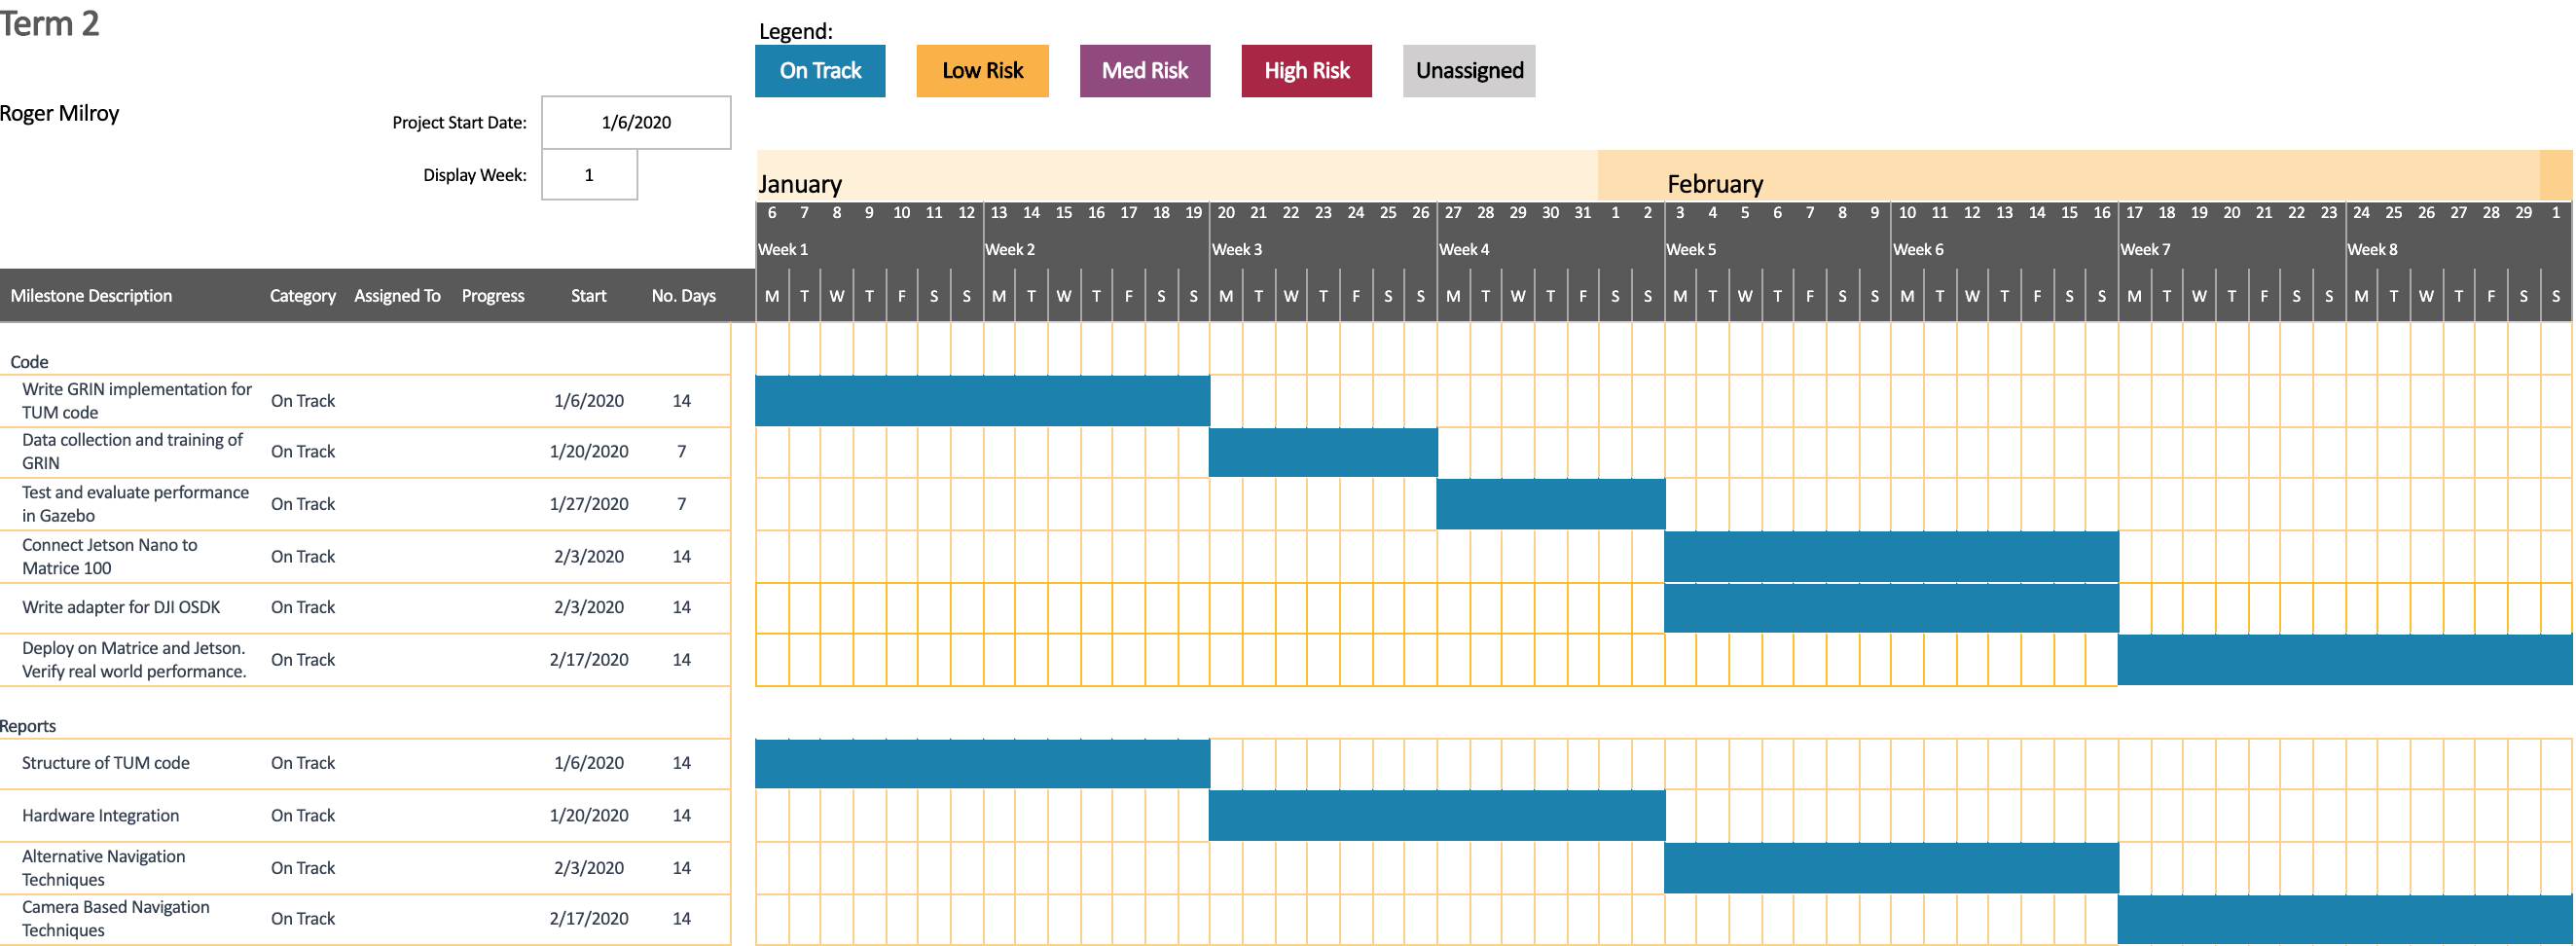
\includegraphics[width=\textwidth]{Term2GanttChart.png}  
  \caption{Term 2 Gantt Chart.}
  \label{}
\end{figure}

%%%%%%%%%%%%%%%%%
%%%% BIBLIOGRAPHY

\newpage
\bibliographystyle{acm}
\bibliography{../resources/final_project}
\nocite{*}

\label{endpage}

\begin{appendices}

  \chapter{Project Diary}
  
  Monday October 7: Learned about ROS topics and publishers. Created two simple example programs. One to make a simple robot travel in a circle, one to stop. Appears that publishing once to the /cmd\_vel topic does not have any effect. Appears that it needs to be sent multiple times.
  
  Wednesday October 9: I set up the git repo both on my main device and the VM in which I will be working mostly. I added the Project Plan to the Reports folder and generally did some repo management.
  
  Saturday October 12: I have started my report on Kalman Filters. I have read the important parts of the original paper introducing the technique as well as some other explanations. I have written the introduction.
  
  Sunday October 13: I started reading the follow up paper to the original Kalman paper which expands on the technique. I also spent more time understanding the mathematics of the original paper.
  
  Monday October 14: I learned more about publishers and subscribers. I created my catkin workspace. I am having some issues in setting up my development environment how I want it. I want to have ros and gazebo running concurrently and interacting but I am not sure how to get that working. That will be the next thing to work on.
  
  Thursday October 17: I worked on getting the hector\_quadcopter package working. This will be my base for experimentation and work. This took a lot of time and pain. Getting the correct packages in the right place was not simple. This is mainly because the most recent version of ROS and Gazebo are not supported as standard. You have to clone 4 of the tu-darmstadt repos and repeatedly call catkin\_build. One major hiccup I encountered was that at one stage the memory needs expands dramatically and can cause a non-obvious failure. I will detail more on the best installation procedure in separate notes.
  
  Saturday October 19: I finished my report on Kalman Filters. Right now it seems a little too high level so I may return and add in the mathematical content.
  
  Monday October 21: I learnt more about how to connect the Raspberry Pi to the Matrice 100. I found that it is somewhat easier than I expected in some ways and a bit harder in others. There is a cable to connect from the UART on the drone to USB on the RasPi. However I will need some kind of voltage regulator for the power supply. In addition, the interface between ROS on the RasPi and the Matrice and DJI OSDK is not clear yet.
  
  Wednesday October 23: I learned more about Services and how to write Service clients and servers in rospy. I also learned some about writing ROS packages in C++. I think that I will probably end up writing packages in C++ due to performance requirements for my project. I am planning to write demonstrators in rospy and use that to determine whether that will be sufficient. If not I will implement the final deliverables in C++.
  
  Thursday October 24: I reevaluated the project plan, assessed progress so far and revised my milestones for both terms. This has led to a more organised structure to the plan, with more focused proof of concept programs and a more logical structure to second term deliverables. I have now organised them around the implementation details ie. hardware, software or data.
  
  Monday October 28: I started learning about Graph Neural Networks. I found a couple of review papers that should contain a good overview as well as references to specific techniques.
  
  Tuesday October 29: I continued learning about Graph Neural Networks. I have decided to review an online guide that introduces the basic concepts before continuing with the academic papers.
  
  Friday November 1: I started to prepare a Raspberry Pi (Raspi) to run PyTorch and ROS. I updated the version of python to 3.7 which was more effort than I expected due to the way Raspian deals with python. I also researched alternatives to the Raspi in case it is not powerful enough (quite likely). I have decided the best alternative is the Nvidia Jetson due to price (100 pounds) and the fact that it has cuda support which will speed up code execution by a significant factor. It is also compatible with PyTorch out of the box which will simplify my life considerably.
  
  Monday November 4: I finished learning about ROS Actions so I know have all the pieces I need to implement my project from the perspective of ROS. I read the GRIN paper in full so I now have a good idea of what I will be implementing from that point of view. Finally I also learned about PyTorch Geometric which is what I will use to implement the GNN part of the algorithm. I still have much more to learn on that part but I have a good start at this stage.
  
  Wednesday November 6: After meeting with Sara I looked at which version of ROS the TUM code is targeting or working with. It is Indigo so it is likely to need a reasonable amount of work to port to Melodic. I have also decided to push back the report on Graph Neural Networks as it is too broad at this point. I will refocus the report and complete it after one exploring more of the professional issues as well as a report on GRIN, the technique I am looking to implement.
  
  Thursday November 7: I rewrote my Project Plan today to take account of the changed scope and deliverables anticipated. I also finished a first draft of the report on GRIN.
  
  Sunday November 10: I set up the Jetson Nano device. I installed ROS, Gazebo and PyTorch. This means that it is now ready for deploying code once I have integrated it with the Matrice. I also set up my project, cloning and building the libraries that I am using. This was again painful but now I know the pain points I have written a clear and simple guide to getting it up and running.
  
  Thursday November 14: I have forked the TUM repository that I need to port to the current version of ROS and then extend. I attempted to build it on the Jetson Nano. It failed due to a dependency on a package called ardrone\_autonomy. I attempted to install that to satisfy the dependency but it failed. It seems that it can’t be built for ARM architecture which is a problem. It is mainly a wrapper for the Parrot AR SDK. I tried on the VM I have on my laptop as it is amd64 architecture so that would avoid the issues with ARM. It failed for other reasons that seem to require rewriting the library. I abandoned this. I then tried to find all the references to ardrone\_autonomy in the TUM code to remove them. There were not too many. So I decided to replace them where possible.
  
  Friday November 15: I found that most of the references to ardrone\_autonomy are just using messages defined in the ardrone\_autonomy package. I found the definitions and extracted them into a new standalone package called navdata\_msgs. After some work on the CMakeLists.txt file and package.xml it builds successfully. I then replaced all occurences of ardrone\_autonomy with navdata\_msgs. On building I get other errors related to a third party library that the TUM code relies upon. This is called libcvd and it seems to fail on C++ compliant code which is confusing. I tried removing the library from the tarball that it is packaged in and install it from source elsewhere but this still fails. I now know that because I was not cleaning before remaking it was using a cached version so no changes were propagated to the new build.
  
  Saturday November 16: I have tried again to incorporate the new libcvd into the thirdparty tarball. The new version makes fine on its own so I hope that it will be fine if I get the configuration correct. I found that the original had a different folder structure as well as a Makefile that the new one (from GitHub) did not. I replicated the old structure and tried to rebuild and it gets much further than before but now gets stuck linking a header file from the new libcvd. I had to pull over two old files from libcvd-1.0 thread.h and runnable.h as they are used in the TUM code for some reason, it doesn’t affect any other code so it is safe to do this. Also add \#include to cvd/utility.h to fix another bug in the new libcvd version. Currently it doesn’t think that transform is part of the CVD namespace though it seems to be defined to be so in cvd/vision.h. Need to figure that out. This whole process is somewhat exemplary of the difficulties of using old academic projects. There are often serious compatibility issues because they are not maintained. This is the main challenge at this point. Once everything has been built successfully this will hopefully be less of an issue as I can control what is modified and build upon what I have learned about the project structure and CMake. Pretty useful experience though in terms of debugging old make configurations. I had no idea about how CMake worked or how to use it but now I have a pretty good idea.
  
  Sunday 17 November: I finished my report on the applications of GPS Denied Navigation. I fixed the error of transform not being defined in the CVD namespace. It turns out that you need to have CVD\_HAVE\_TOON defined for that function to be defined in the header file. After defining it before import it then works. There is another issue though of Thread not referring to anything as I needed to move the thread.cpp file at the same time as thread.h. Currently having issues in linking the moved files. Getting pretty close to having it work I think though.
  
  Monday November 18: I added the thread header and source files to the CMakeLists.txt. But it didn’t work. I tried to make install TooN. That didn’t work as there was no target for install. Then I tried switching to libcvd 1-x branch. Didn’t work. I removed the GUI Node as I don’t need it and it was causing problems that are not easily reconcilable, potential solutions caused new issues. I found that no thread files or functions were becoming part of the .so file (shared object). From that I found a Makefile I hadn’t looked in before, it was inside libcvd, that added all the .o object files. I added cvd\_src/thread.o to the list and it worked. Added roslib to the CMakeLists.txt and package.xml as it has been separated from roscpp and is needed by one of the functions. Refactored EstimationNode.cpp and .h to remove references to tf and use tf2 instead. This was the final issue as tf has been deprecated. I also had to add tf2 to the dependancies list in CMakeLists.txt. After all that I now have the TUM code building successfully. It took much more time than I wanted but that is unfortunately part of the process. If I had reimplemented it all myself, I would have saved time in debugging build errors but spent much more time in development overall. I think that despite the work it should be worth it. Next is to test the functionality and interface it with the hector drone.
  
  Thursday November 22: I ran the TUM code and it runs with no errors at this point. I started to review the hector stack to see how I can interface the TUM code as the SLAM and controlling node. The hector stack is very large and has lot’s of interdependencies. I am exploring the feasibility of porting the core elements to a package that has less coupling. This is for two reasons. One is to enable the project to be set up more simply and enable easier extension. Second is to reduce overhead so the Jetson has an easier job compiling and running the code. I have not come to a decision yet as it will be non trivial to accomplish due to the interconnectedness.
  
  Saturday November 24: I familiarised myself more with the hector codebase. I have decided that it is not a good idea to try and extract the minimal core elements. The code base is simply too large and interconnected to do in a reasonable amount of time. I will instead modify just one of the packages to interface and work with the TUM code. I have also been thinking about the correct way to incorporate these projects into my github setup. Currently I have forked the repositories that I need to modify and I was planning to add them as submodules but I need to consult Dave to see if that is acceptable. There are alternative solutions that keep all of the project private if that is necessary so I will do that if I need to after consulting Dave.
  
  Sunday November 24: I got the date of the last post wrong. On Sunday I spent more time learning about Graph Neural Networks. I have also found that there is a Distinguished Lecture on the topic of Graph Neural Networks on Monday so I will be going to that and I shall see if it improves my understanding. I will be starting to implement the GRIN this week as well as writing a report on Graph Neural Networks so the timing is very good! I am also starting my interim report in order for it to be mostly complete by the end of the week ready for Sara to read and give feedback on a draft.
  
  Tuesday November 26: I created the dataset for the GRIN or Hybrid Inference implementation. I needed to define a linear model that will generate the data for a simulated system. The maths was not too involved, the only complication is in the discretisation of the equations. After defining the linear model, I added a function that generates a number of samples, returning the ground truth (state) and the measured position. The next step is to define the Kalman filter and then the Hybrid Inference setup. Then training and testing. I am behind schedule but I still expect to complete on time due to the slack I built in to the schedule.
  
  Saturday November 30: I worked out the formulation of the Hybrid Inference technique. This took me a lot more time than expected as I had previously understood that it consisted of a Kalman filter and an additional GNN. That is not actually how it works. They reformulate the Kalman filter as a graph message passing routine that passes messages from past states, future states and observations in order to iteratively improve the estimates of the states. The GNN is then an equivalent graph that has hidden states of x replace x (states). These are randomly initialised. The hidden states of y are the y’s (observations) passed through either a convolution or an MLP to generate the hidden states of y. The picture is of the white board where I worked this all out. I referred to the paper for most of the graphical formulation. For the GNN part I referred to the source code that the authors wrote in addition to the paper. Neither are particularly understandable so there was a lot of referring back and forth and figuring out what was meant.
  
  Sunday December 1: I wrote my own implementation of Hybrid Inference. I referred a lot to the workings I had done on the whiteboard the day before. The GNN implementation was still the most opaque part of the whole technique. There are quite a few tricks and I was trying to write it in a more modular fashion to facilitate using it standalone for comparison purposes. I am not sure that I achieved it but it is at least close and structurally it is modular. I know that it will need some modifications before it will work correctly on its own but they should be minor. The GNN step is something of a mirror of the graphical formulation with the matrix multiplications that compute the messages between nodes replaced by 3 layer neural networks. Then a neural network computes the new hidden states of x and finally in the hybrid formulation there is a decoding step that creates a correction signal epsilon that helps to modify the estimates of x better than the graphical model alone. Testing is the next step to verify that it works as expected followed by training and evaluation.
  
  \end{appendices}
  
\end{document}

\end{article}